
\subsection{Class Distribution}
Figure~\ref{fig:class-dist} shows the distribution of the classes in the training dataset. It's clear that a rating of 2 is by far the most common, followed by 3. However, it's only a 61.2\% majority, which means a model that always guesses 2 won't have the best accuracy.

\begin{figure}[!ht]
    \centering
    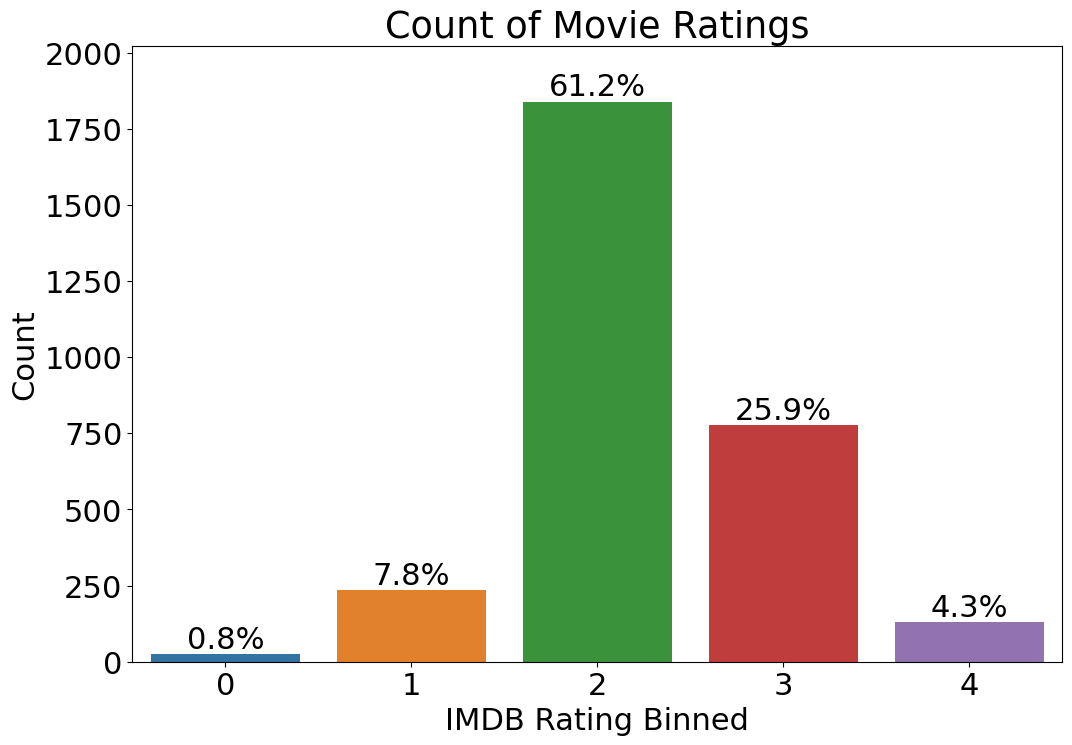
\includegraphics[width = 0.48\textwidth]{res/class-dist.png}
    \caption{Count plot showing the distribution of classes in the training data}
    \label{fig:class-dist}
\end{figure}

\subsubsection{Zero Rule Model}
Based of this class distribution, a 0R model should have approximately a 60\% accuracy, and this will be used as a baseline for the rest of the models.

\subsection{Preprocessing}

\subsubsection{Unhelpful Features}
Since most films are in english and there are many other unique values with very low frequency, the language feature is not very useful and should be dropped. A similar occurence also exists with the country feature, where the USA is an overwhelming majority. 

\ 

\noindent
Similarly, a large majority of movies are either R or PG-13 rated, and so the rating of a movie would not be very helpful and can lead to overfitting. As such \texttt{content\_rating} was also dropped from the dataset.

\subsubsection{Names}
Through filtering out all of the text attributes, we are also filtering out the names of actors and the movie director. Whilst the quality of film can be correlated to its director, and people often enjoy certain movies with certain actors more, the names alone are not enough to generalise the IMDB rating of a movie. This could instead result in the model memorising which directors and actors are better rated, and since there's a limited number of names, would result in overfitting to the training data.


\subsection{Model 1: Support Vector Machine}
The best hyperparameters were found to be:

\textbf{C: } 10

\textbf{Gamma: } 0.01

\textbf{Kernel: } RBF

\noindent
The performance of the model was as below:

\noindent
\textbf{Accuracy on validation set:} 74.3\%

\noindent
\textbf{Cross validation score on all data:} 69.8\%  

\begin{table}[!ht]
    \begin{center}
        \begin{tabular}{c|c|c|c|c}			
            \hline
            Class & Prec. & Recall & F1-Score & Support \\
            \hline\hline
            0 & 0.00 & 0.00 & 0.00 & 5 \\
            1 & 0.00 & 0.00 & 0.00 & 48 \\
            2 & 0.75 & 0.93 & 0.83 & 377 \\
            3 & 0.72 & 0.57 & 0.63 & 152 \\
            4 & 0.75 & 0.47 & 0.58 & 19\\
            \hline
        \end{tabular}

        \caption{\textit{Classification Report of the Best SVM Model without Feature Selection}}
        \label{svm-report}

    \end{center}
\end{table}
\begin{table}[!ht]
    \begin{center}
        \begin{tabular}{c||c|c|c}			
            \hline
             & Prec. & Recall & F1-Score \\
             \hline\hline
            Macro Avg & 0.44 & 0.39 & 0.41 \\
            Weighted Avg & 0.68 & 0.74 & 0.70 \\
            \hline
        \end{tabular}

        \caption{\textit{Summary of Classification Report of the Best SVM Model without Feature Selection}}
        \label{svm-report-sum}

    \end{center}
\end{table}
\begin{figure}[!ht]
    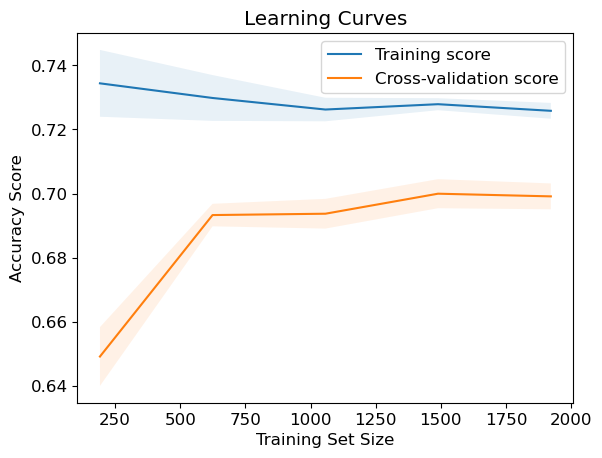
\includegraphics[width = 0.48\textwidth]{res/svm-lc.png}
    \caption{\textit{Learning Curve for the Best SVM Model}}
    \label{fig:svm-lc}
\end{figure}
\noindent
The best feature set found was:
\begin{itemize}
    \item Number of Critics for Reviews
    \item Duration
    \item Director Facebook Likes
    \item Gross
    \item Number of Voted Users
    \item Cast Total Facebook Likes
    \item Face Number in Poster
    \item Title Year
    \item Movie Facebook Likes
    \item Genres
\end{itemize}

\noindent
The performance of the model was as below:

\noindent
\textbf{Accuracy on validation set:} 73.4\%

\noindent
\textbf{Cross validation score on all data:} 73.8\%  

\begin{table}[!ht]
    \begin{center}
        \begin{tabular}{c|c|c|c|c}			
            \hline
            Class & Prec. & Recall & F1-Score & Support \\
            \hline\hline
            0 & 0.00 & 0.00 & 0.00 & 5 \\
            1 & 0.00 & 0.00 & 0.00 & 48 \\
            2 & 0.74 & 0.93 & 0.83 & 377 \\
            3 & 0.70 & 0.54 & 0.61 & 152 \\
            4 & 0.69 & 0.47 & 0.56 & 19\\
            \hline
        \end{tabular}

        \caption{\textit{Classification Report of the Best SVM Model without Feature Selection}}
        \label{svm-ft-report}
    \end{center}
\end{table}

\begin{table}[!ht]
    \begin{center}
        \begin{tabular}{c||c|c|c}			
            \hline
             & Prec. & Recall & F1-Score \\
             \hline\hline
            Macro Avg & 0.43 & 0.39 & 0.40 \\
            Weighted Avg & 0.67 & 0.73 & 0.69 \\
            \hline
        \end{tabular}

        \caption{\textit{Summary of Classification Report of the Best SVM Model without Feature Selection}}
        \label{svm-ft-report-sum}

    \end{center}
\end{table}

\begin{figure}[!ht]
    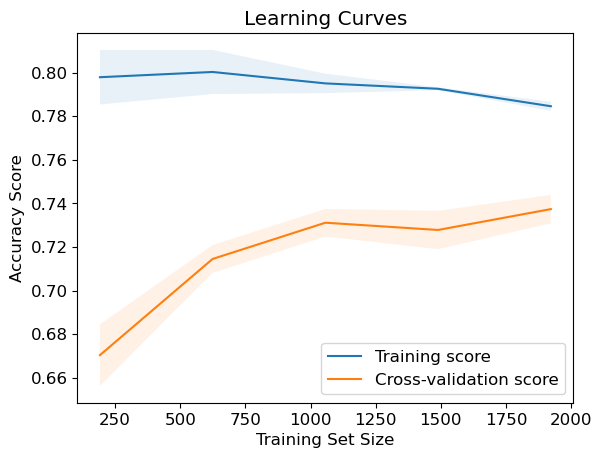
\includegraphics[width = 0.48\textwidth]{res/svm-ft-lc.png}
    \caption{\textit{Learning Curve for the Best SVM Model with Feature Selection}}
    \label{fig:svm-ft-lc}
\end{figure}


\subsection{Model 2: Logistic Regression}
The best hyperparameters were found to be:

\textbf{C: } 0.1

\textbf{Max Iterations: } 1000

\textbf{Penalty: } L2

\textbf{Solver: } Saga

\noindent
The performance of the model was as below:

\noindent
\textbf{Accuracy on validation set:} 65.2\%

\noindent
\textbf{Cross validation score on all data:} 62.7\%  

\begin{table}[!ht]
    \begin{center}
        \begin{tabular}{c|c|c|c|c}			
            \hline
            Class & Prec. & Recall & F1-Score & Support \\
            \hline\hline
            0 & 0.00 & 0.00 & 0.00 & 5 \\
            1 & 0.00 & 0.00 & 0.00 & 48 \\
            2 & 0.65 & 0.99 & 0.79 & 377 \\
            3 & 0.69 & 0.12 & 0.20 & 152 \\
            4 & 0.00 & 0.00 & 0.00 & 19\\
            \hline
        \end{tabular}

        \caption{\textit{Classification Report of the Best Logistic Regression Model without Feature Selection}}
        \label{logr-report}

    \end{center}
\end{table}
\begin{table}[!ht]
    \begin{center}
        \begin{tabular}{c||c|c|c}			
            \hline
             & Prec. & Recall & F1-Score \\
             \hline\hline
            Macro Avg & 0.27 & 0.22 & 0.20 \\
            Weighted Avg & 0.58 & 0.65 & 0.54 \\
            \hline
        \end{tabular}

        \caption{\textit{Summary of Classification Report of the Best Logistic Regression Model without Feature Selection}}
        \label{logr-report-sum}

    \end{center}
\end{table}
\begin{figure}[!ht]
    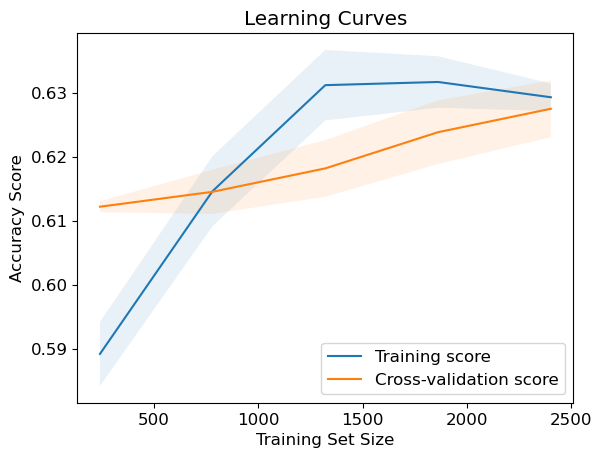
\includegraphics[width = 0.48\textwidth]{res/logr-lc.png}
    \caption{\textit{Learning Curve for the Best Logistic Regression Model}}
    \label{fig:logr-lc}
\end{figure}
\noindent
The best feature set found was:
\begin{itemize}
    \item Number of Critics for Reviews
    \item Duration
    \item Director Facebook Likes
    \item Gross
    \item Number of Voted Users
    \item Cast Total Facebook Likes
    \item Genres
\end{itemize}
\noindent
The performance of the model was as below:

\noindent
\textbf{Accuracy on validation set:} 72.0\%

\noindent
\textbf{Cross validation score on all data:} 62.9\%  

\begin{table}[!ht]
    \begin{center}
        \begin{tabular}{c|c|c|c|c}			
            \hline
            Class & Prec. & Recall & F1-Score & Support \\
            \hline\hline
            0 & 0.00 & 0.00 & 0.00 & 5 \\
            1 & 0.00 & 0.00 & 0.00 & 48 \\
            2 & 0.72 & 0.95 & 0.82 & 377 \\
            3 & 0.71 & 0.44 & 0.54 & 152 \\
            4 & 0.89 & 0.42 & 0.57 & 19\\
            \hline
        \end{tabular}

        \caption{\textit{Classification Report of the Best Logistic Regression Model without Feature Selection}}
        \label{logr-ft-report}

    \end{center}
\end{table}
\begin{table}[!ht]
    \begin{center}
        \begin{tabular}{c||c|c|c}			
            \hline
             & Prec. & Recall & F1-Score \\
             \hline\hline
            Macro Avg & 0.46 & 0.36 & 0.39 \\
            Weighted Avg & 0.66 & 0.72 & 0.67 \\
            \hline
        \end{tabular}

        \caption{\textit{Summary of Classification Report of the Best Logistics Regression Model without Feature Selection}}
        \label{logr-ft-report-sum}

    \end{center}
\end{table}
\begin{figure}[!ht]
    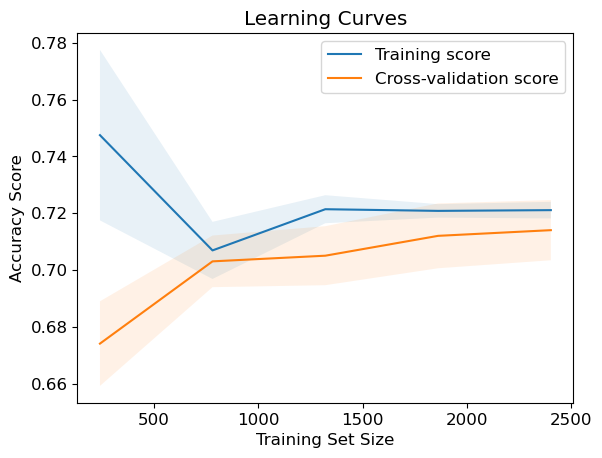
\includegraphics[width = 0.48\textwidth]{res/logr-ft-lc.png}
    \caption{\textit{Learning Curve for the Best Logistic Regression Model with Feature Selection}}
    \label{fig:logr-ft-lc}
\end{figure}


\subsection{Model 3: Random Forest}
The model was seeded using the seed 42.

The best hyperparameters were found to be:

\textbf{Max Depth: } 10

\textbf{N Estimators: } 100

\textbf{Max Features: } Auto


\noindent
The performance of the model was as below:

\noindent
\textbf{Accuracy on validation set:} 70.7\%

\noindent
\textbf{Cross validation score on all data:} 71.2\%  

\begin{table}[!ht]
    \begin{center}
        \begin{tabular}{c|c|c|c|c}			
            \hline
            Class & Prec. & Recall & F1-Score & Support \\
            \hline\hline
            0 & 0.00 & 0.00 & 0.00 & 5 \\
            1 & 0.00 & 0.00 & 0.00 & 48 \\
            2 & 0.72 & 0.92 & 0.81 & 377 \\
            3 & 0.64 & 0.45 & 0.53 & 152 \\
            4 & 0.62 & 0.42 & 0.50 & 19\\
            \hline
        \end{tabular}

        \caption{\textit{Classification Report of the Best Random Forest Model without Feature Selection}}
        \label{rf-report}

    \end{center}
\end{table}
\begin{table}[!ht]
    \begin{center}
        \begin{tabular}{c||c|c|c}			
            \hline
             & Prec. & Recall & F1-Score \\
             \hline\hline
            Macro Avg & 0.40 & 0.36 & 0.37 \\
            Weighted Avg & 0.64 & 0.71 & 0.66 \\
            \hline
        \end{tabular}

        \caption{\textit{Summary of Classification Report of the Best Random Forest Model without Feature Selection}}
        \label{rf-report-sum}

    \end{center}
\end{table}
\begin{figure}[!ht]
    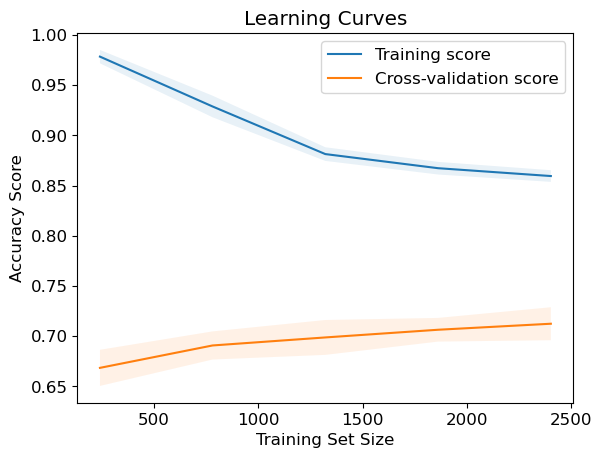
\includegraphics[width = 0.48\textwidth]{res/rf-lc.png}
    \caption{\textit{Learning Curve for the Best Random Forest Model}}
    \label{fig:rf-lc}
\end{figure}
\noindent
The best feature set found was:
\begin{itemize}
    \item Number of Critics for Reviews
    \item Duration
    \item Director Facebook Likes
    \item Gross
    \item Number of Voted Users
    \item Cast Total Facebook Likes
    \item Title Year
    \item Movie Facebook Likes
    \item Average Degree of Centrality
    \item Genres
\end{itemize}

\noindent
The performance of the model was as below:

\noindent
\textbf{Accuracy on validation set:} 70.4\%

\noindent
\textbf{Cross validation score on all data:} 72.0\%  

\begin{table}[!ht]
    \begin{center}
        \begin{tabular}{c|c|c|c|c}			
            \hline
            Class & Prec. & Recall & F1-Score & Support \\
            \hline\hline
            0 & 0.00 & 0.00 & 0.00 & 5 \\
            1 & 0.00 & 0.00 & 0.00 & 48 \\
            2 & 0.74 & 0.94 & 0.83 & 377 \\
            3 & 0.69 & 0.51 & 0.59 & 152 \\
            4 & 0.67 & 0.32 & 0.43 & 19\\
            \hline
        \end{tabular}

        \caption{\textit{Classification Report of the Best Random Forest Model without Feature Selection}}
        \label{rf-ft-report}

    \end{center}
\end{table}
\begin{table}[!ht]
    \begin{center}
        \begin{tabular}{c||c|c|c}			
            \hline
             & Prec. & Recall & F1-Score \\
             \hline\hline
            Macro Avg & 0.42 & 0.35 & 0.37 \\
            Weighted Avg & 0.66 & 0.73 & 0.68 \\
            \hline
        \end{tabular}

        \caption{\textit{Summary of Classification Report of the Best Random Forest Model without Feature Selection}}
  27      \label{rf-ft-report-sum}

    \end{center}
\end{table}
\begin{figure}[!ht]
    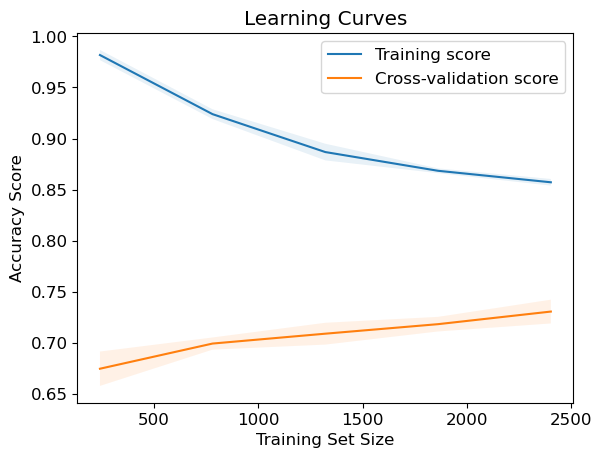
\includegraphics[width = 0.48\textwidth]{res/rf-ft-lc.png}
    \caption{\textit{Learning Curve for the Best Random Forest Model with Feature Selection}}
    \label{fig:rf-ft-lc}
\end{figure}

